\chapter{绪论}

交互设计是一种设计并定义人造系统内多个个体间交流的内容与结构,使之互相配合,以达成某种目的的行为。交互设计早在 20 世纪 80 年代就作为一门新兴学科诞生了,但直到进入 21 世纪后,软件界面相比传统硬件界面交互信息层级更为复杂,交互方式更为多样化,交互设计才从网页设计和图形设计中独立开来,成为一个专门的领域。让用户更为高效、准确地进行交互操作,完成使用目的,并得到交互过程中的愉悦感,这是交互设计的根本目的。交互设计当前主要的设计领域包括网页、移动端操作系统和应用、电脑操作系统和应用和其他终端系统及应用等。

全景漫游是当今互联网行业发展最为迅速的技术之一,它是虚拟现实(即 VR 技术)的基础。沉浸性和交互性是其得到众多用户青睐的最主要原因,可供用户身临其境般体验的图形化界面,以及不同于传统平面媒介的交互手段共同促进了全景漫游技术的推广。

全景漫游解决了传统工业界对于空间概念呈现形式不足的痛点,通过定义场景的 360 度无缝全景图像,仿佛使人置身于制作者脑海中设计出的环境内,配合移动设备内置陀螺仪支持的重力感应功能,足不出户即可感受任何可以用图像表达的场景。80 天环游地球不再只是一个梦想,而且现今全景播放设备层出不穷,最便宜的 Google Cardboard 制作成本不足一元钱,人人 VR 的时代即将到来。

\section{研究背景}
当前交互设计的研究重点大多数着眼于基于平面屏幕设备的交互过程,比如手机屏幕上的交互等。屏幕交互的特点是:显示屏幕形态为矩形较为规则,人与屏幕的距离较远,屏幕的可视区域不会随着视线的改变而改变等。而全景漫游所支持的设备屏幕为两个凸透镜状镜片,用户所观察到的“屏幕”边界不明显,可以通过转动头部进行改变视角视野的观察,这与一般的交互设计的设计主体有了明显的不同。并且全景漫游中信息层级被刻意弱化了,但强调了场景的完整性,这一点与传统的以页面层级对用户信息界面进行划分的交互形式也有所区别。如何利用全景漫游合理地布置交互元素,并构建合理的交互形式以期符合用户的认知模型,从而让用户在使用全景漫游时能够高效愉悦地进行体验,是全景漫游中交互设计所研究的重点。

\begin{figure}[htp]
\centering
\fbox{
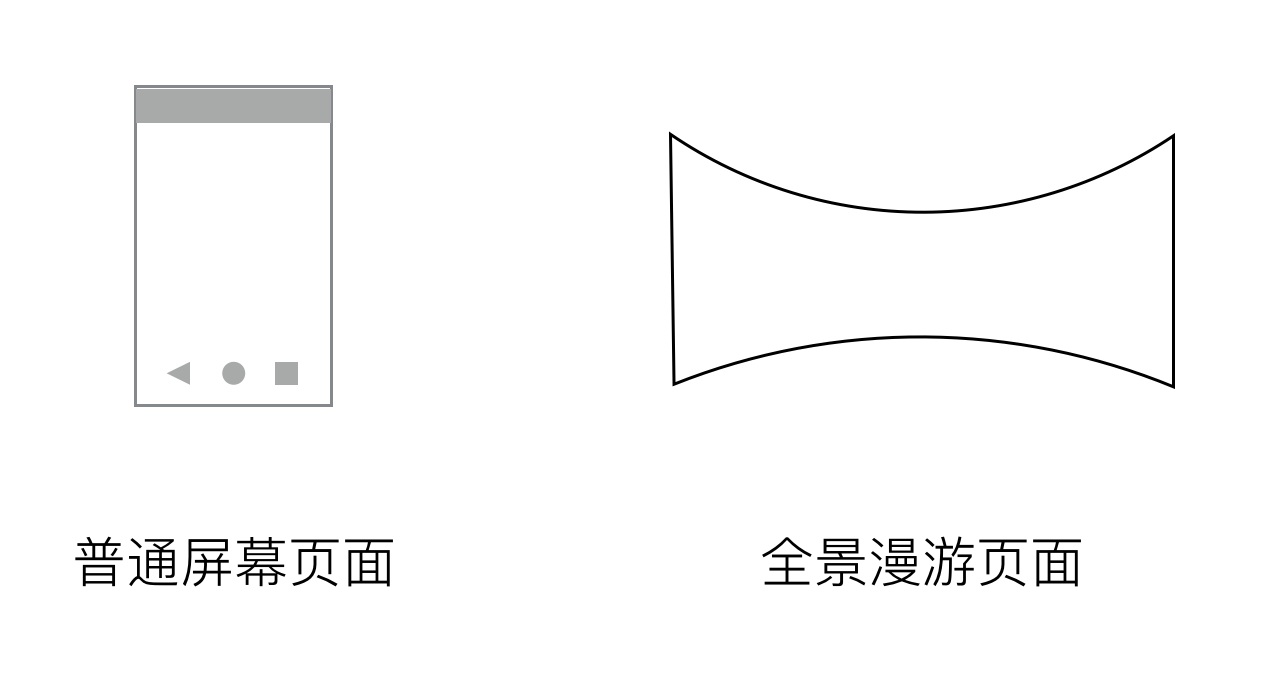
\includegraphics[width=.5\textwidth]{screen}
}
\caption{普通屏幕页面与全景漫游界面}
\label{fig:screen}
\end{figure}

交互设计领域当前已有相当多的研究成果,例如人机交互界面(即 HCI)相关学科和理论一直是国际上计算机相关学科研究的重点,辛向阳教授将人与系统交互的过程分解为了五个要素,分别为:用户、行为、目标、场景、媒介(peopl、actions、means、purpose、contexts)。拥有良好的科研氛围和市场实践经验,交互设计的学科体系已然较为成熟。再看到全景漫游这一方面,其计算机相关理论也较为成熟,相关的图像信号捕捉处理算法已被大范围应用与实践中,各种根据特殊用途产生的适配处理也增强了全景漫游相关应用的鲁棒性。例如,在敦煌石窟数字化工作中的洞窟全景漫游技术初步应用一文\endnote{宋利良,李大丁. 敦煌石窟数字化工作中的洞窟全景漫游技术初步应用[J]. 敦煌研究,2010,(06):93-97.}中,作者以高动态范围影像( HDR)处理为例说明了敦煌石窟在拍摄全景图像至后期处理中遇到的难点和问题。

与技术成熟相对的是,全景漫游方面的交互研究一直停留在起步阶段。在中国知网(cnki.net)上搜索“全景漫游 设计”,命中 359 条结果,搜索“全景漫游 技术“,命中 712 条结果。其中,“全景漫游 设计”的命中结果中有大部分为“程序设计”的相关论文,故可以得出国内相关设计研究尚未达到成熟,全景漫游相关设计理论仍有较大的发展空间。如何将全景漫游的技术应用到交互设计中,将两者有机结合,扩展交互设计的应用领域。

\section{研究目的}
本研究试图扩展交互设计的应用领域,将全景漫游中原本简单易见的场景架构扩充为复杂的漫游系统架构,适宜用户利用全景漫游进行包括但不限于场景漫游的操作。从交互角度解释全景漫游中各组件的作用,利用交互设计中的信息架构模型和交互模型等思想,分析全景漫游中相应模型与传统界面的区别之处,并结合人机工程学的观点对人在漫游中的作用进行探究。研究将以理论结合实践,借鉴实际应用中已经成熟的交互方案,从用户为中心的角度出发进行整体架构及布局,并通过实际项目设计进行案例分析深入探讨理论应用于实践的形式。

\section{研究内容}
本文采用以文献阅读法为基础,采用规范研究法为主要研究方法,通过已知现象和经验为基础,以理论推导相关实践形式的价值判断,并据此完成相关设计工作,最后以定量分析和定性分析结合的形式对全景漫游中可视化交互理论成果进行检验。

研究范围为全景漫游与人的关系(从人机工程学和认知心理学角度进行分析)、全景漫游的多通道交互形式、全景漫游的信息架构、功能模型与交互模型、全景漫游可视化交互的评价体系。

本文研究步骤如下

\begin{description}
\item[第一部分] 通过文献阅读、资料检索及市场调查的方式对市面上已有的全景漫游产品及技术进行整理分析,概括全景漫游发展趋势及现状。

\item[第二部分] 从人出发,通过结合人机工程学及认知心理学的观点,对人进行全景漫游中所遇到的与一般界面交互不同的行为进行比较,并探究全景漫游中技术上具有可行性、并且与人的常规认知所匹配的交互形式。

\item[第三部分] 以界面所共有的信息架构为研究对象,从信息组织形式角度出发,阐述交互设计在全景漫游中所需要解决的实际问题。针对全景漫游设计其特有的交互形式,提取出交互模型以作设计参考。

\item[第四部分] 将以前文所梳理的全景漫游中可视化设计的理论知识为基础,以项目为设计对象通过需求定义、功能分析、设计模型、原型设计的方式进行设计实践。

\item[第五部分] 通过定量分析和定性分析的双重方法建立全景漫游中可视化交互设计的设计评价标准,并对前文中设计实例进行试评价。

\end{description}

\section{研究意义}
交互设计起源之初仅仅考虑使用键盘和鼠标进行交互操作的形式,直至进入移动时代,人们习惯于使用手指直接触摸屏幕操作,交互的内容和形式均得到了扩充。与用户所见到的交互界面不同,设计师在进行设计时所建立的信息架构与交互模型在屏幕界面上是隐形的,故交互设计的意义在于通过隐式的模型建立出实际可行的显式的交互形式。

研究全景漫游的可视化交互的意义在于:
\begin{enumerate}
	\item 将交互设计引入全景漫游的体验中,有助于建立科学有效的交互模型,从架构层面改善优化全景漫游的应用体验,增强用户的使用满意度
	\item 全景漫游的发展长期依赖于技术的进步,而忽视了设计在其中所占的重要作用。建立基于全景漫游技术的可视化交互理论,能够将技术与设计有机地结合起来,互取所长。
	\item 将全景漫游相关设计理论补充入交互设计中形成反哺,可以拓展交互设计的应用领域,利用实践增强其可信性。
\end{enumerate}

